\chapter{central force motion solutions}
\begin{abox}
	Practice set 1 solutions
	\end{abox}
\begin{enumerate}
	\begin{minipage}{\textwidth}
		\item The acceleration due to gravity $(g)$ on the surface of Earth is approximately $2.6$ times that on the surface of Mars. Given that the radius of Mars is about one half the radius of Earth, the ratio of the escape velocity on Earth to that on Mars is approximately
		\exyear{NET JUNE 2011}
	\end{minipage}
	\begin{tasks}(2)
		\task[\textbf{A.}] $1.1$
		\task[\textbf{B.}]$1.3$
		\task[\textbf{C.}]$2.3$
		\task[\textbf{D.}]$5.2$
	\end{tasks}
\begin{answer}
	$\text { Escape velocity }=\sqrt{2 g R}$\\
	$\frac{\text { Escape velocity of Earth }}{\text { Escape velocity of Mass }}=\sqrt{\frac{g_{e} R_{e}}{g_{m} R_{m}}}=2.3 \quad \text { where } \frac{R_{e}}{R_{m}}=2 \text { and } \frac{g_{e}}{g_{m}}=2.6$\\
	THe correct option is \textbf{(c)}
\end{answer}
\begin{minipage}{\textwidth}
	\item Two particles of identical mass move in circular orbits under a central potential $V(r)=\frac{1}{2} k r^{2}$. Let $l_{1}$ and $l_{2}$ be the angular momenta and $r_{1}, r_{2}$ be the radii of the orbits respectively. If $\frac{l_{1}}{l_{2}}=2$, the value of $\frac{r_{1}}{r_{2}}$ is:
	\exyear{NET DEC 2011}
\end{minipage}
\begin{tasks}(2)
	\task[\textbf{A.}] $\sqrt{2}$
	\task[\textbf{B.}]$1 / \sqrt{2}$
	\task[\textbf{C.}] 2
	\task[\textbf{D.}] $1 / 2$
\end{tasks}
\begin{answer}
	 $V_{e f f}=\frac{l^{2}}{2 m r^{2}}+\frac{1}{2} k r^{2}$, where $l$ is angular momentum.\\\\
	Condition for circular orbit $\frac{\partial V_{e f f}}{\partial r}=0 \Rightarrow-\frac{l^{2}}{m r^{3}}+k r=0 \Rightarrow l^{2} \propto r^{4} \Rightarrow l \propto r^{2}$.\\
	Thus $\frac{l_{1}}{l_{2}}=\left(\frac{r_{1}}{r_{2}}\right)^{2} \Rightarrow \frac{r_{1}}{r_{2}}=\sqrt{\frac{l_{1}}{l_{2}}} \Rightarrow \frac{r_{1}}{r_{2}}=\sqrt{2}$\\ since $\frac{l_{1}}{l_{2}}=2$.\\
	The correct option is \textbf{(a)}
\end{answer}
\begin{minipage}{\textwidth}
	\item A planet of mass $m$ moves in the inverse square central force field of the Sun of mass $M$. If the semi-major and semi-minor axes of the orbit are $a$ and $b$, respectively, the total energy of the planet is:
	\exyear{NET DEC 2011}
\end{minipage}
\begin{tasks}(2)
	\task[\textbf{A.}] $-\frac{G M m}{a+b}$
	\task[\textbf{B.}]$-G M m\left(\frac{1}{a}+\frac{1}{b}\right)$
	\task[\textbf{C.}]$-\frac{G M m}{a}\left(\frac{1}{b}-\frac{1}{a}\right)$
	\task[\textbf{D.}]$-G M m\left(\frac{a-b}{(a+b)^{2}}\right)$
\end{tasks}
\begin{answer}
 Assume Sun is at the centre of elliptical orbit. Conservation of energy\\
  $\frac{1}{2} m v_{1}^{2}-\frac{G M m}{a}=\frac{1}{2} m v_{2}^{2}-\frac{G M m}{b}$\\ Conservation of momentum $L=m v_{1} a=m v_{2} b$\\
  \begin{figure}[H]
  	\centering
  	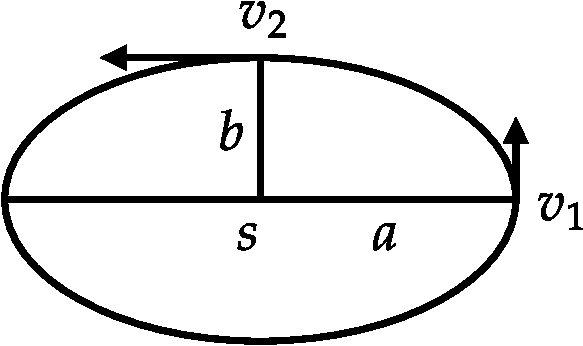
\includegraphics[height=3cm,width=5cm]{diagram-20210926(12)-crop}
  \end{figure}
 \begin{align*}
 	&v_{2}=v_{1}\left(\frac{a}{b}\right) \\
 	&\frac{1}{2} m v_{1}^{2}-\frac{1}{2} m v_{2}^{2}=\frac{G M m}{a}-\frac{G M m}{b} \Rightarrow \frac{1}{2} m\left(v_{1}^{2}-v_{1}^{2} \frac{a^{2}}{b^{2}}\right)=G M m\left(\frac{b-a}{a b}\right) \\
 	&\frac{1}{2} m v_{1}^{2}\left(\frac{b^{2}-a^{2}}{b^{2}}\right)=G M m\left(\frac{b-a}{a b}\right) \Rightarrow \frac{1}{2} m v_{1}^{2}=G M m\left(\frac{b}{a}\right) \cdot \frac{1}{(b+a)} \\
 	&E=\frac{1}{2} m v_{1}^{2}-\frac{G M m}{a}=G M m \frac{b}{a} \frac{1}{(b+a)}-\frac{G M m}{a} \\
 	&=\frac{G M m}{a}\left(\frac{b}{(b+a)}-1\right)=\frac{G M m}{a}\left(\frac{b-b-a}{(b+a)}\right)=-\frac{G M m}{(b+a)}
 \end{align*}
 The correct option is \textbf{(a)}	
\end{answer}
\begin{minipage}{\textwidth}
	\item A planet of mass $m$ moves in the gravitational field of the Sun (mass $M$ ). If the semimajor and semi-minor axes of the orbit are $a$ and $b$ respectively, the angular momentum of the planet is
	\exyear{NET DEC 2012}
\end{minipage}
\begin{tasks}(2)
	\task[\textbf{A.}]$\sqrt{2 G M m^{2}(a+b)}$
	\task[\textbf{B.}]$\sqrt{2 G M m^{2}(a-b)}$
	\task[\textbf{C.}]$\sqrt{\frac{2 G M m^{2} a b}{a-b}}$
	\task[\textbf{D.}]$\sqrt{\frac{2 G M m^{2} a b}{a+b}}$
\end{tasks}
\begin{answer}
	 Assume Sun is at the centre of elliptical orbit.\\\\
	Conservation of energy $\frac{1}{2} m v_{1}^{2}-\frac{G M m}{a}=\frac{1}{2} m v_{2}^{2}-\frac{G M m}{b}$\\\\
	Conservation of momentum $L=m v_{1} a=m v_{2} b$
	$$
	v_{2}=v_{1}\left(\frac{a}{b}\right)
	$$
	\begin{figure}[H]
		\centering
		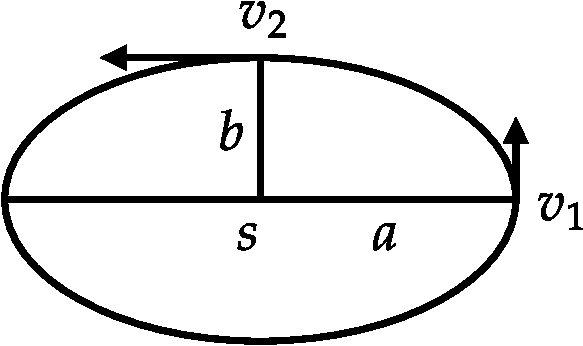
\includegraphics[height=3cm,width=5cm]{diagram-20210926(12)-crop}
	\end{figure}
	\begin{align*}
		&\frac{1}{2} m v_{1}^{2}-\frac{1}{2} m v_{2}^{2}=\frac{G M m}{a}-\frac{G M m}{b} \Rightarrow \frac{1}{2} m\left(v_{1}^{2}-v_{1}^{2} \frac{a^{2}}{b^{2}}\right)=G M m\left(\frac{b-a}{a b}\right) \\
		&\frac{1}{2} m v_{1}^{2}\left(\frac{b^{2}-a^{2}}{b^{2}}\right)=G M m\left(\frac{b-a}{a b}\right) \Rightarrow \frac{1}{2} m v_{1}^{2}=G M m\left(\frac{b}{a}\right) \cdot \frac{1}{(b+a)} \\
		&v_{1}=\sqrt{2 G M\left(\frac{b}{a}\right) \cdot \frac{1}{(b+a)}} \\
		&L=m v_{1} a=m \sqrt{2 G M\left(\frac{b}{a}\right) \cdot\left(\frac{1}{b+a}\right)} \cdot a=m \sqrt{\frac{2 G M a b}{(b+a)}} \Rightarrow L=\sqrt{\frac{2 G M m^{2} a b}{a+b}}
	\end{align*}
	The correct option is \textbf{(d)}
\end{answer}
\begin{minipage}{\textwidth}
	\item A planet of mass $m$ and an angular momentum $L$ moves in a circular orbit in a potential, $V(r)=-k / r$, where $k$ is a constant. If it is slightly perturbed radially, the angular frequency of radial oscillations is
	\exyear{NET JUNE 2013}
\end{minipage}
\begin{tasks}(2)
	\task[\textbf{A.}] $m k^{2} / \sqrt{2} L^{3}$
	\task[\textbf{B.}]$m k^{2} / L^{3}$
	\task[\textbf{C.}]$\sqrt{2} m k^{2} / L^{3}$
	\task[\textbf{D.}]$\sqrt{3} m k^{2} / L^{3}$
\end{tasks}
\begin{answer}$\left. \right. $\\
	\begin{minipage}{0.5\textwidth}
	$V_{e f f}=\frac{L^{2}}{2 m r^{2}}-\frac{k}{r} .$\\
	For circular orbit $\frac{\partial V_{e f f}}{\partial r}=-\frac{L^{2}}{m r^{3}}+\frac{k}{r^{2}}=0$ \\
	$\Rightarrow \frac{L^{2}}{m r^{3}}=\frac{k}{r^{2}} .$ \\
	Thus $r=r_{0}=\frac{L^{2}}{m k} \Rightarrow \omega=\sqrt{\frac{k}{m}}$,
	\end{minipage}
\begin{minipage}{0.5\textwidth}
\begin{figure}[H]
	\centering
	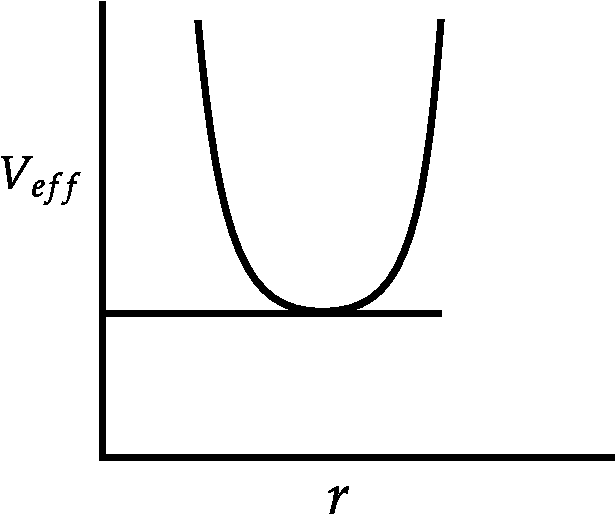
\includegraphics[height=4cm,width=5cm]{diagram-20210926(17)-crop}
\end{figure}
\end{minipage}
 $$k=\left.\frac{d^{2} V_{e f f}}{d r^{2}}\right|_{r=r_{0}}=+\frac{3 L^{2}}{m r^{4}}-\left.\frac{2 k}{r^{3}}\right|_{r=r_{0}}=\frac{3 L^{2}}{m\left(\frac{L^{2}}{m k}\right)^{4}}-\frac{2 k}{\left(\frac{L^{2}}{m k}\right)^{3}}=\frac{3 m^{3} k^{4}}{L^{6}}-\frac{2 m^{3} k^{4}}{L^{6}}=\frac{m^{3} k^{4}}{L^{6}}$$
 $$\omega=\sqrt{\frac{\left.\frac{d^{2} V}{d r^{2}}\right|_{r=r_{0}}}{m}} \Rightarrow \omega=\frac{m k^{2}}{L^{3}}$$
 The correct option is \textbf{(b)}	
\end{answer}

\end{enumerate}